\section{Practica: Ejercicio Modelo de Dominio Inspectores}

\begin{figure}[!htb]
    \centering
    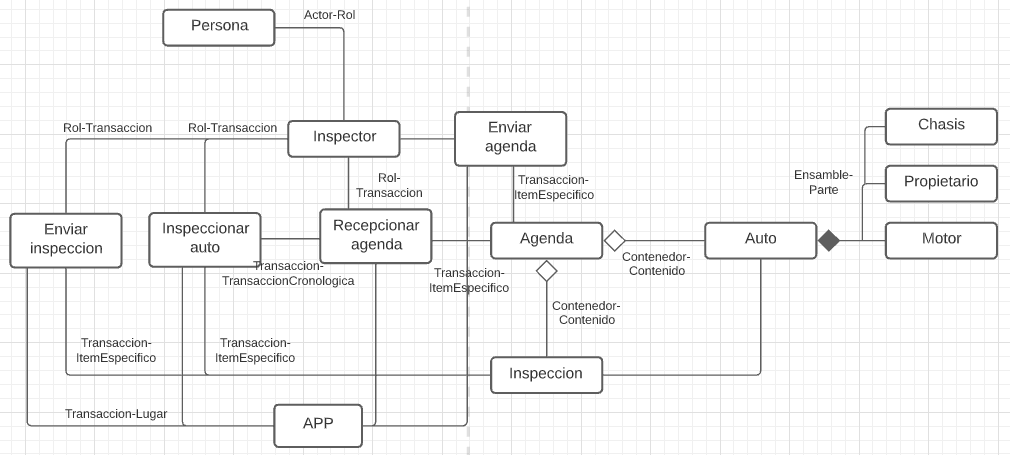
\includegraphics[width=\textwidth]{img/EjercicioInspectores.PNG}
\end{figure}

\begin{itemize}
\item Seguir los pasos para resolver el ejercicio. Empezar con Actor-Rol y seguir a partir de ahi.
\item No pensar en la implementación.
\item Se esta narrando como el inspector lleva adelante su trabajo.
\item No tiene sentido una Transacción sin un Item.
\item Nos interesan cuestiones del negocio en la resolución del ejercicio. \textit{Que se pueda cancelar algo ahora no es relevante.}
\item Inspección-Auto tiene una relación directa.
\end{itemize}

\subsection*{Ejemplo Sandwich}

\begin{figure}[!htb]
    \centering
    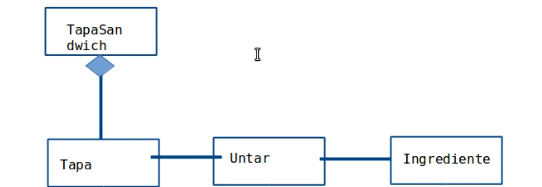
\includegraphics[width=0.6\textwidth]{img/ModeloSandwich.PNG}
\end{figure}

El siguiente ejemplo de código esta mal, no representa correctamente el modelo que se planteo para el sándwich.
\begin{minted}
[
frame=leftline,
framesep=5mm,
baselinestretch=1.2,
]
{java}
Sandwich s = new Sandwich();
Tapa t1 = new Tapa()
Tapa t2 = new Tapa()
Ingrediente i = new Ingrediente()

t1.set(i)
s.set(t1)
s.set(t2)
...
\end{minted}

Este en cambio, respeta el modelo planteado.
\begin{minted}
[
frame=leftline,
framesep=5mm,
baselinestretch=1.2,
]
{java}
Tapa t1 = new Tapa()
Tapa t2 = new Tapa()
Ingrediente i = new Ingrediente()
i.untar(t1)
Sandwich s = t2.montar(t1)
...
\end{minted}